\documentclass[a4paper, % A4
	parskip, % Absätze durch Abstand statt Einrückung gekennzeichnet
	%draft, % überlange Zeilen werden nicht%markiert
	ngerman, % english, hyphenation etc.
    numbers=noenddot] % no trailing period after headings
	{scrreprt} % Report (KOMA-Script)

% redefine old commands used by the glossary plugin
\makeatletter
\DeclareOldFontCommand{\rm}{\normalfont\rmfamily}{\mathrm}
\DeclareOldFontCommand{\sf}{\normalfont\sffamily}{\mathsf}
\DeclareOldFontCommand{\tt}{\normalfont\ttfamily}{\mathtt}
\DeclareOldFontCommand{\bf}{\normalfont\bfseries}{\mathbf}
\DeclareOldFontCommand{\it}{\normalfont\itshape}{\mathit}
\DeclareOldFontCommand{\sl}{\normalfont\slshape}{\@nomath\sl}
\DeclareOldFontCommand{\sc}{\normalfont\scshape}{\@nomath\sc}
\makeatother

\usepackage{fontspec}

\usepackage[babel]{microtype} % Automatische Grauwertverbesserung
\usepackage[ngerman]{babel} % warning that option english is not loaded yet
    % when not declaring [USenglish] even though documentclass sets it globally
\usepackage{IEEEtrantools} % bibliography, quoting (\cite)

\usepackage{graphicx} % include images (\includegrafics)
\usepackage[section]{placeins} % place floating objects before a \FloatBarrier

\usepackage{framed} % frame paragraphs (\begin{framed})
\usepackage[left=2.54cm,right=2.54cm,bottom=2.54cm,top=2.54cm]{geometry} % change margin for title page (\newgeometry, % \resetgeometry)
\usepackage{setspace} % change line spacing (\onehalfspacing)
\usepackage{pdflscape} % pages in landscape (\begin{landscape})
\usepackage{multicol} % multiple columns for a sector (\begin{multicols})

\usepackage{booktabs} % Professional looking tables (\toprule,% \midrule,
	% \bottomrule)
\usepackage{threeparttable} % table with notes (\tnote, \begin{tablenotes})
\usepackage[table]{xcolor}
\usepackage{longtable}

\usepackage{amsmath}
\usepackage{array}
\newenvironment{conditions}[1][wobei:]
  {#1 \begin{tabular}[t]{>{$}l<{$} @{${}={}$} l}}
  {\end{tabular}\\[\belowdisplayskip]}

\usepackage{enumitem}

\newenvironment{itquote}
  {\begin{quote}\itshape}
  {\end{quote}\ignorespacesafterend}

\usepackage{pgfplots} % charts
\pgfplotsset{compat=1.13}
\usetikzlibrary{patterns}

% Redefine space before and after chapter title
\renewcommand*{\chapterheadstartvskip}{\vspace*{12pt}}
\renewcommand*{\chapterheadendvskip}{\vspace*{12pt}}

\usepackage[printonlyused, % show only used acronyms
		% withpage, % show pagenumber of first usage
	] % longform in footnote (instead of shortform)
	{acronym} % abbreviations  (\ac, \acs,\acl)
		% \begin{acronym})
		
\usepackage{pdfpages} % include PDFs (\includepdf)
\usepackage{float} % own floating objects (\newfloat, \floatname)

% \nameref)
%rename the output for an \autoref{chap:XXX} from lowercase chapter to Chapter
% and also for Section and Subsection
\addto\extrasUS{%
  \renewcommand{\chapterautorefname}{Chapter}% 
}
\addto\extrasUSenglish{%
  \renewcommand{\sectionautorefname}{Section}% 
}
\addto\extrasUSenglish{%
  \renewcommand{\subsectionautorefname}{Subsection}% 
}

\setcounter{secnumdepth}{3}

% Roman numerals for chapter
\renewcommand{\thechapter}{\Roman{chapter}}
\renewcommand{\thesection}{\arabic{section}}
% global formatting
\onehalfspacing % 1.5x line spacing

% count figures and labels continuously
% hot fix for chnngcntr https://tex.stackexchange.com/questions/425600/latex-error-command-counterwithout-already-defined
\let\counterwithout\relax
\let\counterwithin\relax
\usepackage{chngcntr}
\counterwithout{figure}{chapter}
\counterwithout{table}{chapter}

\usepackage{color}

%Package for syntax highlighting (needs pygments installed): https://tex.stackexchange.com/a/256796
\usepackage{caption}
\usepackage{minted}
\captionsetup[listing]{}
\captionsetup{labelfont=bf}

% Default options for code listing
\setminted[python]{linenos, frame=leftline, numbersep=8pt, framesep=8pt, tabsize=4}

\setminted[sql]{frame=leftline, numbersep=8pt, framesep=8pt, tabsize=4}

% bigger line numbers for code blocks
\renewcommand{\theFancyVerbLine}{\sffamily {\small \oldstylenums{\arabic{FancyVerbLine}}}}

\usepackage{hyperref} % linking to refs and URLs (\ref, \url, \autoref, \hyperref)

\usepackage{datatool}
\usepackage[toc, nonumberlist, nopostdot]{glossaries}

\emergencystretch 3em

\usepackage{fancyhdr} % headings on each page
\pagestyle{fancy}
\renewcommand{\headrulewidth}{0pt}

% rename "Kapitel" in header to "Teil"
\makeatletter
\renewcommand{\@chapapp}{Teil}
\makeatother
\newcommand{\code}[1]
	{\texttt{#1}}
\newcommand{\command}[1]
    {\textit{#1}}
\newcommand{\filepath}[1]
	{\texttt{#1}}
\newcommand*{\fullref}[1]
    {\hyperref[{#1}]{\autoref*{#1} \nameref*{#1} on page \pageref*{#1}}}
\newcommand{\linenumber}[1]
    {\textit{#1}}
\newcommand{\productname}[1]
	{\textit{#1}}
\newcommand{\tbd}[1]
    {{\color{red}<tbd> #1}}
\newfloat{listingfloat}{htb}{qcl}[chapter]
\floatname{listingfloat}{Listing}
\newcommand{\nextitem}{\par\hspace*{\labelsep}\textbullet\hspace*{\labelsep}} % bulletpoints in a table cell: Source: https://tex.stackexchange.com/a/54048
% definiton of frequenlty used standard texts.
% Usage in text: \authors{} -> Jonas Matter, Robin Suter

\newcommand{\authors}
	{Jonas Matter, Robin Suter}
\newcommand{\place}
	{HSR Hochschule für Technik Rapperswil \\Institut für Software}
\newcommand{\timeperiod}
	{12. Juni 2018}
\newcommand{\titel}
	{ÖV-Güteklassen 2018}
\newcommand{\subtitel}
    {} %TODO
\newcommand{\work}
	{Spezifikation}


\loadglsentries{appendix/glossary}
\makeglossaries
\glsaddall

\begin{document}
\setromanfont[BoldFont={Gentium Basic Bold},ItalicFont={Gentium Basic Italic}]{Gentium Basic}

% Following the template unter www.hsr.ch > HSR-intern > Bachelor-Studiengänge
% > Informatik > allgemeine Infos Diplom-, Bachelor- und Studienarbeiten.

\newgeometry{left=2.25cm, right=2.25cm, top=2.25cm, bottom=2.25cm} % new
% margins

\begin{titlepage}

\begin{center}
\begin{minipage}[t]{0.45\textwidth}
    
\includegraphics[width=\textwidth]{start/img/hsrLogo}
\end{minipage}
\hspace{\fill} % horizontal space
\begin{minipage}[t]{0.45\textwidth}
    \vspace{-2.56cm}
    
\includegraphics[width=\textwidth]{start/img/ifsLogo}
\end{minipage}

\end{center}

\vspace{15ex} % vertical space
\Huge
\textbf{\titel}

% \vspace{1ex}
\huge
\textbf{\subtitel}

\vspace{4ex}
\textbf{\work}

\vspace{1ex}
\LARGE 
\place

\vspace{5ex}
\timeperiod

\vspace{11ex}
\begin{tabular}{ll} % Table
	Autoren:        & \authors    \\
\end{tabular}

\end{titlepage}

\restoregeometry % reset page margins

\begin{quote}
      
    \thispagestyle{empty}
    \newlength\longest
    \null\vfill
    
    \settowidth\longest{\huge\itshape Wenden wir uns der Vergangenheit zu,}
    \centering
    \parbox{\longest}{%
        \raggedright{\huge\itshape%
            Wenden wir uns der Vergangenheit zu, \\ 
            das wird ein Fortschritt sein\par\bigskip
        }   
        \raggedleft{"`Tornate all'antico e sarà un progresso"', schrieb Giuseppe Verdi am 5. Januar 1871 an Francesco Florimo}\par%
    }
    
    \vfill\vfill
    
    \clearpage
    
\end{quote}

\addcontentsline{toc}{chapter}{Inhaltsverzeichnis}
\tableofcontents

\chapter{Einführung}
\label{Einführung}

\section{Grundlagen und Begriffe}
\label{Einführung:Grundlagen und Begriffe}

Nachfolgend werden Grundlagen und Begriffe eingeführt, welche für das grundlegende Verständnis des Dokuments relevant sind. Für zusätzliche Definitionen kann das Glossar zur Hand gezogen werden.

\subsection{ÖV-Güteklasse}
\label{Grundlagen und Begriffe:ÖV-Güteklasse}

\subsubsection{Definition}
% same description is used in the corresponding glossary entry
"`\acs{ÖV}-Güteklassen geben Auskunft darüber, wie gut ein Standort mit dem öffentlichen Verkehr erschlossen ist.
Dies ist wichtig, wenn es darum geht, den öffentlichen Verkehr zu optimieren, Siedlungsverdichtung nach Innen an geeigneten Lagen voranzutreiben oder Standortentscheide für publikumsintensive Anlagen so zu treffen, dass sie möglichst wenig zusätzlichen Autoverkehr verursachen."'~\cite{oev-guteklasse-gr-defintion}

\subsubsection{OeVGK93}
% same description is used in the corresponding glossary entry
OeVGK93 steht kurz für \acs{ÖV}-Güteklassen 93 und bezeichnet die Definition der \acs{ÖV}-Güteklassen, welche im Jahre 1993 mit der \acs{SN} 640 290~\cite{sn640290} verabschiedet wurde.

\subsubsection{OeVGK18}
% same description is used in the corresponding glossary entry
OeVGK steht kurz für \acs{ÖV}-Güteklassen 2018 und bezeichnet die neue Spezifikation der \acs{ÖV}-Güteklassen, welche in diesem Dokument beschrieben wird.

\cleardoublepage
\section{Dank}
\label{Resultate:Dank}

Wir möchten folgenden Personen für ihre Unterstützung und Mitwirkung beim Erarbeiten dieser Spezifikation danken:

\textbf{Prof. Stefan Keller, IFS Institut für Software}

\textbf{Prof. Claudio Büchel, IRAP Institut für Raumentwicklung}
% Summary index document for ...

\chapter{Technischer Bericht}
\label{Technischer Bericht}


\section{Stand der Technik}
\label{Stand der Technik}

\subsection{Aktuelle Situation}
\label{Stand der Technik:Aktuelle Situation}

\subsubsection{Schweizer Norm 640 290}
\label{Aktuelle Situation:Schweizer Norm 640 290}

\acs{ÖV}-Güteklassen wurden erstmals mit der \ac{SN} 640 290~\cite{sn640290} des Vereins Schweizerischer Strassenfachleute (VSS) im Jahre 1993 für die Schweiz definiert.
Diese Norm enthält Richtwerte für die Bestimmung des Grenzbedarfs an Parkfeldern für Personenwagen und führte hierfür die Definition der \acs{ÖV}-Güteklassen ein.
Im Jahre 2006 wurde diese durch die \acs{SN} 640 281 abgelöst, welche nicht mehr auf die \acs{ÖV}-Güteklassen eingeht.
Es wurde seither keine allgemeingültige Definition verabschiedet.

Im Folgenden ist aufgeschlüsselt, was genau die \acs{SN} 640 290~\cite{sn640290} in Bezug auf \acs{ÖV}-Güteklassen definiert und wo Schwachstellen liegen.

\paragraph{Definition ÖV-Güteklassen}~\\
\label{Schweizer Norm 640 290:Definition ÖV-Güteklassen}
Grundsätzlich definieren \acs{ÖV}-Güteklassen die Qualität der Erschliessung durch den öffentlichen Verkehr.
Diese Qualität wird durch die \nameref{Definition ÖV-Güteklassen:Bedienungsqualität der Haltestelle} und die \nameref{Definition ÖV-Güteklassen:Erreichbarkeit der Haltestelle} festgesetzt.
Beide Kriterien sind folgend definiert.
Anmerken muss man, dass zu besserer Verständlichkeit und Übersichtlichkeit unter anderem zusätzliche Terminologie wie Verkehrsmittelkategorie eingeführt wird.

\subparagraph{Bedienungsqualität der Haltestelle}~\\
\label{Definition ÖV-Güteklassen:Bedienungsqualität der Haltestelle}
Die öffentlichen Verkehrsmittel werden zuerst in Verkehrsmittelkategorien eingeteilt:

\begin{itemize}[noitemsep]
    \item Verkehrsmittelkategorie 1
    \begin{itemize}
        \item Bahnknoten: mehrere Bahnlinien in unterschiedliche Richtungen
    \end{itemize}
    \item Verkehrsmittelkategorie 2
    \begin{itemize}
        \item Bahnlinie
    \end{itemize}
    \item Verkehrsmittelkategorie 3
    \begin{itemize}
        \item Tramway, Trolleybuy, Autobus, Regionalbus, Ortsbus mit gutem Anschluss an Bahnlinie
    \end{itemize}
    \item Verkehrsmittelkategorie 4
    \begin{itemize}
        \item Ortsbus, lokaler Kleinbus
    \end{itemize}
\end{itemize}

Die Verkehrsmittelkategorien werden dabei in die Gruppe A und B zusammengefasst, welche für die Berechnung des durchschnittlichen Kursintervalls berücksichtigt werden.
Dabei werden für die Intervallberechnung alle Verkehrsmittel der Verkehrsmittelkategorie in einer Gruppe berücksichtigt.

\begin{table}[ht]
    \begin{tabular}[c]{l | p{2.9cm} p{2.9cm} | p{2.9cm} p{2.9cm}}
        \toprule
        \textbf{Kursintervall}
                                & \multicolumn{4}{c}{\textbf{Verkehrsmittelkategorie}}\\
        \midrule
        \textbf{}
                                & \multicolumn{2}{c|}{\textbf{Gruppe A}}
                                & \multicolumn{2}{c}{\textbf{Gruppe B}}\\
        \textbf{}
                                & \textbf{1}
                                & \textbf{2}
                                & \textbf{3}
                                & \textbf{4}\\
        \textbf{< 5 min}
                                & I
                                & I
                                & II
                                & III\\
        \textbf{5 -- 9 min}
                                & I
                                & II
                                & III
                                & IV\\
        \textbf{10 -- 19 min}
                                & II
                                & III
                                & IV
                                & V\\
        \textbf{20 -- 39 min}
                                & III
                                & IV
                                & V
                                & V\\
        \textbf{40 -- 60 min}
                                & IV
                                & V
                                & V
                                & -\\
        \bottomrule
    \end{tabular}
    \caption{Ermittlung der Haltestellenkategorie}
    \label{table:Ermittlung der Haltestellenkategorie}
\end{table}

Der Kursintervall ist der durchschnittliche Abstand zwischen Ankunft beziehungsweise Abfahrt (pro Linie jeweils in der Hauptlastrichtung) aller Verkehrsmittel in der gleichen Gruppe zwischen 06:00 -- 20:00 Uhr jeweils von Montag bis Freitag.
Die Norm macht hier Ausnahmen bei Verdichtungen in Hauptverkehrszeiten, Linienüberlagerungen und reinen Arbeitsplatzgebieten mit stark verdichtetem Fahrplan während Pendlerzeiten.

\subparagraph{Erreichbarkeit der Haltestelle}~\\
\label{Definition ÖV-Güteklassen:Erreichbarkeit der Haltestelle}
Basierend auf den vorhin definierten Haltestellenkategorien (I bis V) kann die Erreichbarkeit pro Haltestellenkategorien definiert werden.
Die Distanzen sind Luftlinien, wobei ein mittlerer Umwegfaktor von 20 bis 30\% berücksichtigt wird.

\begin{table}[ht]
    \begin{tabular}[c]{l p{2.5cm} p{2.5cm} p{2.5cm} p{2.5cm}}
        \toprule
        \textbf{Haltestellenkategorie}
                                & \multicolumn{4}{c}{\textbf{Distanz zur Haltestelle}}\\
        \midrule
        \textbf{}
                                & \textbf{< 300 m}
                                & \textbf{300 -- 500 m}
                                & \textbf{501 -- 750 m}
                                & \textbf{751 -- 1000m}\\
        \textbf{I}
                                & Klasse A
                                & Klasse A
                                & Klasse B
                                & Klasse C\\
        \textbf{II}
                                & Klasse A
                                & Klasse B
                                & Klasse C
                                & Klasse D\\
        \textbf{III}
                                & Klasse B
                                & Klasse C
                                & Klasse D
                                & -\\
        \textbf{IV}
                                & Klasse C
                                & Klasse D
                                & -
                                & -\\
        \textbf{V}
                                & Klasse D
                                & -
                                & -
                                & -\\
        \bottomrule
    \end{tabular}
    \caption{Ermittlung der Erreichbarkeit der Haltestelle}
    \label{table:Ermittlung Erreichbarkeit der Haltestelle}
\end{table}

Der Topographie wird Rechnung getragen, indem man bei schwierigen Gegebenheiten die nächste Klasse wählt oder die Distanz vergrössert.

\subsection{Lösungsansätze}
\label{Stand der Technik:Lösungsansätze}
Basierend auf der bestehenden \nameref{Aktuelle Situation:Schweizer Norm 640 290} wurde im Jahre 2011 die Berechnungsmethodik des \ac{ARE} veröffentlicht, welche in einer Weisung des \acs{UVEK} vom 16.02.2015 als die Berechnugsmethodik definiert wird, welche bei der Beurteilung der Qualität der Erschliessung mit dem öffentlichen Verkehr verwendet werden soll.

In der Zwischenzeit wurden einige kantonale Anpassungen an dieser Methodik und der \nameref{Aktuelle Situation:Schweizer Norm 640 290} vorgenommen.
Folgend werden grob die Abweichungen der Norm der verabschiedeten Berechnungsmethodik ARE und zweier kantonaler Methodiken beschrieben, namentlich des Kanton Graubünden und Zürich.
Ebenfalls wird ein Blick auf eine österreichische Umsetzung der \acs{ÖV}-Güteklassen geworfen.
% TODO Grundlagenbericht erwähnen

Im Anschluss werden die Methodiken zusammen betrachtet, Schwachstellen eruiert und Verbesserungen vorgeschlagen.
Dieses Vorgehen hat das Ziel, Erfahrungen und etablierte Grundlagen in \gls{OeVGK18} im Kapitel \ref{Spezifikation OeVGK18} einfliessen zu lassen, um so eine allgemeine Akzeptanz erreichen zu können.

\subsubsection{Berechnungsmethodik ARE}
\label{Lösungsansätze:Berechnungsmethodik ARE}
Das Bundesamt für Raumentwicklung (ARE) entwickelt in ihrem Grundlagenbericht für die Beurteilung der Agglomerationsprogramme Verkehr und Siedlung~\cite{berechnung_are} eine Berechnungsmethodik der \acs{ÖV}-Güteklassen basierend auf der bestehende Norm (siehe Kapitel \ref{Aktuelle Situation:Schweizer Norm 640 290}).
Die entwickelte Berechnungsmethodik basiert auf den Fahrplandaten von HAFAS~\cite{sbb_hafas_spec}.
Dies hatte die Konsequenz, dass die Berechnungsmethodik wie sie in der Norm festgelegt ist, angepasst werden musste.
Im Folgenden sind die Anpassungen aufgeführt.

\paragraph{Bedienungsqualität der Haltestelle}~\\
\label{Berechnungsmethodik ARE:Bedienungsqualität der Haltestelle}
Die Verkehrsmittel lassen sich aus dem elektronischen Fahrplan~\cite{sbb_hafas_spec} nicht detailliert unterscheiden, wie es die Norm verlangt.
Dies hat die Konsequenz, dass nur folgenden Verkehrsmittel-Einteilung verwendet wird:

\begin{itemize}[noitemsep]
    \item Verkehrsmittelgruppe A
    \begin{itemize}
        \item Bahnknoten (mehrere Bahnlinien in verschiedenen Richtungen)
        \item Bahnlinien
    \end{itemize}
    \item Verkehrsmittelgruppe B
    \begin{itemize}
        \item Tram, Busse, Postautos, Rufbusse oder Schiffe
    \end{itemize}
    \item Verkehrsmittelgruppe C
    \begin{itemize}
        \item Seilbahnen
    \end{itemize}
\end{itemize}

Die Hauptlastrichtung kann aus den Fahrplandaten nicht extrahiert werden.
Somit werden alle Abfahrten zwischen 6.00 und 20.00 Uhr gezählt und anschliessend halbiert. Bei Endhaltestellen und Linien, welche nur in eine Richtung verlaufen, erfolgen Korrekturen.
Die genaue Art der Korrektur ist nicht weiter aufgeführt.
Als Stichtag für die Auswertung wird ein Werktag ausserhalb der Ferienzeit und der touristischen Hochsaison definiert.
Ebenfalls wir in reinen Arbeitsplatzgebieten mangels einheitlicher Definition keine Anpassung vorgenommen.
Verdichtungen in den Hauptverkehrszeiten sind in den gezählten Abfahrten inbegriffen.

\paragraph{Erreichbarkeit der Haltestelle}~\\
\label{Berechnungsmethodik ARE:Erreichbarkeit der Haltestelle}
Der Topografie wird keine Rechnung getragen, um eine landesweite Vergleichbarkeit sicherzustellen.

Die \acs{ÖV}-Güteklassen sind folgend zu interpretieren:

\begin{itemize}[noitemsep]
    \item Güteklasse A: Sehr gute Erschliessung
    \item Güteklasse B: Gute Erschliessung
    \item Güteklasse B: Mittelmässige Erschliessung
    \item Güteklasse D: Geringe Erschliessung
    \item Keine Güteklasse: Marginale oder keine \acs{ÖV}-Erschliessung
\end{itemize}

\subsubsection{Berechnungsmethodik Kanton Graubünden}
\label{Lösungsansätze:Berechnungsmethodik Kanton Graubünden}
Im technischen Bericht "`Definition \acs{ÖV}-Struktur / Erhebung  \acs{ÖV}-Güteklassen Kanton Graubünden"'~\cite{oev-guteklasse-gr} werden Anpassungen der in der Norm beschriebenen Berechnungsmethodik der \acs{ÖV}-Güteklassen an die speziellen Bedürfnisse des Kanton Graubündens aber auch von allgemeiner Natur vorgenommen.
Anpassungen, welche spezielle Gegebenheiten des Kanton Graubündens betreffen, werden in der folgenden Zusammenstellung ausgeklammert, da sie sich für eine automatische Berechnung und für eine nationale Betrachtung nicht eignen.

\paragraph{Bedienungsqualität der Haltestelle}~\\
\label{Berechnungsmethodik Kanton Graubünden:Bedienungsqualität der Haltestelle}
Es werden zwei zusätzliche Haltestellenkategorieren (VI und VII) ergänzt und eine feinere Gliederung der Taktfrequenz eingeführt.

Auf die Unterscheidung zwischen "`Tram, Trolleybus, Autobus, Regionalbus"' und "`Ortsbus, lokaler Kleinbus"' wird verzichtet und in der ersteren Kategorie zusammengefasst.
Ebenfalls werden Seilbahnen mit Erschliessungsfunktion wie Bushaltestellen behandelt.

\begin{table}[ht]
    \begin{tabular}[c]{l p{4.0cm} p{4.0cm} p{4.0cm}}
        \toprule
        \textbf{Kursintervall}
                                & \multicolumn{3}{c}{\textbf{Art des Verkehrsmittels}}\\
        \midrule
        \textbf{}
                                & \textbf{Bahnknoten}
                                & \textbf{Bahnlinie}
                                & \textbf{Tram/Bus}\\
        \textbf{< 5 min}
                                & I
                                & I
                                & II\\
        \cellcolor{red!25}\textbf{5 -- 10 min}
                                & I
                                & II
                                & III\\
        \cellcolor{red!25}\textbf{11 -- 19 min}
                                & II
                                & III
                                & IV\\
        \textbf{20 -- 39 min}
                                & III
                                & IV
                                & V\\
        \textbf{40 -- 60 min}
                                & IV
                                & V
                                & \cellcolor{red!25}VI\\
        \cellcolor{red!25}\textbf{> 60 min}
                                & -
                                & \cellcolor{red!25}VII
                                & \cellcolor{red!25}VII\\
        \bottomrule
    \end{tabular}
    \caption{Ermittlung der Haltestellenkategorie Kanton Graubünden}
    \label{table:Ermittlung der Haltestellenkategorie Kanton Graubünden}
\end{table}

Somit werden nun Bushaltestellen, die halbstündlich und stündlich bedient werden, nicht mehr gleich kategorisiert.
Auch werden Haltestellen erfasst, welche seltener als stündlich einen Anschluss haben.
Durch die feinere Gliederung der Taktfrequenz erhält man eine bessere Güteklasse bei einem 10-Minuten-Takt im Vergleich mit einem 15-Minuten-Takt.

\paragraph{Erreichbarkeit der Haltestelle}~\\
\label{Berechnungsmethodik Kanton Graubünden:Erreichbarkeit der Haltestelle}
Die zusätzlichen Haltestellenkategorien (VI und VII) hat zur Folge, dass auch zusätzliche Güteklassen (E und F) eingeführt werden.

\begin{table}[ht]
    \begin{tabular}[c]{l p{2.5cm} p{2.5cm} p{2.5cm} p{2.5cm}}
        \toprule
        \textbf{Haltestellenkategorie}
                                & \multicolumn{4}{c}{\textbf{Distanz zur Haltestelle}}\\
        \midrule
        \textbf{}
                                & \textbf{< 300 m}
                                & \textbf{300 -- 500 m}
                                & \textbf{501 -- 750 m}
                                & \textbf{751 -- 1000m}\\
        \textbf{I}
                                & Klasse A
                                & Klasse A
                                & Klasse B
                                & Klasse C\\
        \textbf{II}
                                & Klasse A
                                & Klasse B
                                & Klasse C
                                & Klasse D\\
        \textbf{III}
                                & Klasse B
                                & Klasse C
                                & Klasse D
                                & -\\
        \textbf{IV}
                                & Klasse C
                                & Klasse D
                                & -
                                & -\\
        \textbf{V}
                                & Klasse D
                                & -
                                & -
                                & -\\
        \cellcolor{red!25}\textbf{VI}
                                & \cellcolor{red!25}Klasse E
                                & -
                                & -
                                & -\\
        \cellcolor{red!25}\textbf{VII}
                                & \cellcolor{red!25}Klasse F
                                & -
                                & -
                                & -\\                                
        \bottomrule
    \end{tabular}
    \caption{Ermittlung der Erreichbarkeit der Haltestelle Kanton Graubünden}
    \label{table:Ermittlung Erreichbarkeit der Haltestelle Kanton Graubünden}
\end{table}

Bushaltestellen haben eine maximale Erschliessungswirkung von 500 Meter, da grössere Distanzen von Passagieren als zu lange empfunden wird.
Somit werden nur Bahnknoten und Bahnlinien in den Kategorien > 500 Meter klassifiziert.
Die Topografie wird manuell berücksichtigt.

Hauptverkehrszeiten werden nicht gesondert gehandhabt.
Es zählt grundsätzlich das Angebot im gegebenen Zeitbereich.

Linien, welche grundsätzlich stündlich fahren, jedoch Taktlücken aufweisen um zu einen gewissen Zeitpunkt ein Angebot erfüllen zu können, werden nur in der Stundentakt-Gruppe klassifiziert, wenn sie nicht mehr als 2 Taktlücken aufweisen.

Es existieren Linienüberlagerungen mit einer ungleichen Verteilung.
So können zwei Linien stündlich verkehren und eine Haltestelle kurz nacheinander bedienen, welche dann als Halbstundentakt klassifiziert werden.
Der Passagier nimmt das Angebot aber als Stundentakt wahr.
Jedoch ist nicht weiter ersichtlich, wie das Problem behoben wird.

Die Bestimmung der Hauptlastrichtung erfolgt analog zur Berechnungsmethodik ARE.

% Brauchen uns Hinketakte zu interessieren und müssen wir das auflisten?

\subsubsection{Berechnungsmethodik Kanton Zürich}
\label{Lösungsansätze:Berechnungsmethodik Kanton Zürich}
Im Infoblatt "`ÖV-Güteklassen"'~\cite{oev-guteklassen-zh} wird beschrieben, wie der Kanton Zürich die kantonalen ÖV-Güteklassen mit den Fahrplandaten des Zürcher Verkehrsverbundes (ZVV), angelehnt an die Berechnungsmethodik \acs{ARE}, berechnet.

\paragraph{Bedienungsqualität der Haltestelle}~\\
\label{Berechnungsmethodik Kanton Zürich:Bedienungsqualität der Haltestelle}
Es werden nur Haltestellen berücksichtigt, die von Bahn, Tram und/oder Bus bedient werden.
Seilbahnen und Schiffe werden explizit ausgeklammert.
Somit ergibt sich folgende Kategorisierung:
\begin{itemize}
    \itemsep -1.5em
    \item Bahnknoten (Bahnstationen mit S-Bahnlinien in min. 6 Richtungen und/oder IR-Anschluss)
    \item Bahnlinien
    \item Tram
    \item Bus
\end{itemize}

Der Kursintervall wird auf 05:30 bis 22:30 Uhr festgelegt (unter der Woche).
Handelt es sich um Endhaltestellen oder Linien, welche nur in eine Richtung verkehren, werden alle Abfahrten gezählt.
Zusätzlich werden wie im Kanton Graubünden  Haltestellen mit einem Kursintervall von über 60 Minuten berücksichtigt.

\begin{table}[ht]
    \begin{tabular}[c]{l p{2.9cm} p{2.8cm} p{2.8cm} p{2.8cm}}
        \toprule
        \textbf{Kursintervall}
                                & \multicolumn{4}{c}{\textbf{Art des Verkehrsmittels}}\\
        \midrule
        \textbf{}
                                & \textbf{Bahnknoten}
                                & \textbf{Bahnlinie}
                                & \textbf{Tram}
                                & \textbf{Bus}\\
        \textbf{< 5 min}
                                & I
                                & I
                                & II
                                & II\\
        \textbf{5 -- 9 min}
                                & I
                                & II
                                & III
                                & III\\
        \textbf{10 -- 19 min}
                                & II
                                & III
                                & IV
                                & IV\\
        \textbf{20 -- 39 min}
                                & III
                                & IV
                                & -
                                & V\\
        \textbf{40 -- 60 min}
                                & -
                                & V
                                & -
                                & VI\\
        \cellcolor{red!25}\textbf{> 60 min}
                                & -
                                & -
                                & -
                                & \cellcolor{red!25}VII\\
        \bottomrule
    \end{tabular}
    \caption{Ermittlung der Haltestellenkategorie Kanton Zürich}
    \label{table:Ermittlung der Haltestellenkategorie Kanton Zürich}
\end{table}


\paragraph{Erreichbarkeit der Haltestelle}~\\
\label{Berechnungsmethodik Kanton Zürich:Erreichbarkeit der Haltestelle}
Auch im Kanton Zürich werden durch den zusätzlich abgebildeten Kursintervall (> 60 Minuten) zwei neue Güteklassen E und F eingeführt.

\begin{table}[ht]
    \begin{tabular}[c]{l p{2.5cm} p{2.5cm} p{2.5cm} p{2.5cm}}
        \toprule
        \textbf{Haltestellenkategorie}
                                & \multicolumn{4}{c}{\textbf{Distanz zur Haltestelle}}\\
        \midrule
        \textbf{}
                                & \textbf{< 300 m}
                                & \textbf{300 -- 500 m}
                                & \textbf{501 -- 750 m}
                                & \textbf{751 -- 1000m}\\
        \textbf{I}
                                & Klasse A
                                & Klasse A
                                & Klasse B
                                & Klasse C\\
        \textbf{II}
                                & Klasse A
                                & Klasse B
                                & Klasse C
                                & Klasse D\\
        \textbf{III}
                                & Klasse B
                                & Klasse C
                                & Klasse D
                                & -\\
        \textbf{IV}
                                & Klasse C
                                & Klasse D
                                & \cellcolor{red!25}Klasse E
                                & -\\
        \textbf{V}
                                & Klasse D
                                & \cellcolor{red!25}Klasse E
                                & \cellcolor{red!25}Klasse E
                                & -\\
        \cellcolor{red!25}\textbf{VI}
                                & \cellcolor{red!25}Klasse E
                                & \cellcolor{red!25}Klasse E
                                & -
                                & -\\
        \cellcolor{red!25}\textbf{VII}
                                & \cellcolor{red!25}Klasse F
                                & \cellcolor{red!25}Klasse F
                                & -
                                & -\\                                
        \bottomrule
    \end{tabular}
    \caption{Ermittlung der Erreichbarkeit der Haltestelle Kanton Zürich}
    \label{table:Ermittlung Erreichbarkeit der Haltestelle Kanton Zürich}
\end{table}

Der Topografie wird keine Rechnung getragen, es wird strikt auf die Luftlinie gesetzt.
Sind Haltestellen nur durch Tram und/oder Bus erschlossen, werden analog zum Kanton Graubünden nur Distanzen bis zu 500 Meter berücksichtigt.
Die Erschliessung durch Bahnknoten und Bahnlinien wird bis 750 Meter mit den Güteklassen B -- E und bis 1000 Meter mit den Güteklassen C --D berücksichtigt.
Diese Entscheidungen basieren auf ÖV-Angebotsverordnungen.

\subsubsection{Berechnungsmethodik Österreich}
\label{Lösungsansätze:Berechnungsmethodik Österreich}

Im Artikel "`\acs{ÖV}-Güteklassen – ein Werkzeug zur Analyse der 
Versorgung eines Standortes mit ÖV"'~\cite{berechnung_oesterreich} ist die Umsetzung der Analyse der Versorgung eines Standortes mit öffentlichem Verkehr in Österreich beschrieben.

\paragraph{Bedienungsqualität der Haltestelle}~\\
\label{Berechnungsmethodik Österreich:Bedienungsqualität der Haltestelle}
Die Kursintervallberechnung erfolg analog zur \nameref{Lösungsansätze:Berechnungsmethodik ARE}.
Herauszuheben ist, dass zwei Stichtage definiert werden, ein gewöhnlicher Werktag und einen Tag, welcher ein besonders ungünstigen Verkehrstag wiederspiegelt.

Es wird keine grundsätzliche Unterscheidung zwischen Bahnknoten und Bahnlinien gezogen, sondern der Fernverkehr wird als das beste mögliche Verkehrsmittel angesehen.

\begin{table}[ht]
    \begin{tabular}[c]{l p{2.9cm} p{2.8cm} p{2.8cm} p{2.8cm}}
        \toprule
        \textbf{Kursintervall}
                                & \multicolumn{4}{c}{\textbf{Art des Verkehrsmittels}}\\
        \midrule
        \textbf{}
                                & \textbf{Fernverkehr REX}
                                & \textbf{S-Bahn, U-Bahn, \dots}
                                & \textbf{Strassenbahn, Metrobus, \dots}
                                & \textbf{Bus}\\
        \textbf{< 5 min}
                                & I
                                & I
                                & II
                                & \cellcolor{red!25}III\\
        \textbf{5 -- 9 min}
                                & I
                                & II
                                & III
                                & III\\
        \textbf{10 -- 19 min}
                                & II
                                & III
                                & IV
                                & IV\\
        \textbf{20 -- 39 min}
                                & III
                                & IV
                                & \cellcolor{red!25}V
                                & V\\
        \textbf{40 -- 60 min}
                                & \cellcolor{red!25}IV
                                & V
                                & \cellcolor{red!25}VI
                                & VI\\
        \cellcolor{red!25}\textbf{60 -- 120 min}
                                & \cellcolor{red!25}V
                                & \cellcolor{red!25}VI
                                & \cellcolor{red!25}VII
                                & \cellcolor{red!25}VII\\
        \cellcolor{red!25}\textbf{121 -- 210 min}
                                & -
                                & \cellcolor{red!25}VII
                                & \cellcolor{red!25}VIII
                                & \cellcolor{red!25}VIII\\
        \bottomrule
    \end{tabular}
    \caption{Ermittlung der Haltestellenkategorie Österreich}
    \label{table:Ermittlung der Haltestellenkategorie Österreich}
\end{table}

Es werden 3 weitere Haltestellenkategorien eingeführt und eine erweiterte Gliederung der Kursintervalle vorgenommen.
So fliegen Haltestellen mit einem Intervall grösser 210 Minuten grundsätzlich bereits aus der Analyse.

\paragraph{Erreichbarkeit der Haltestelle}~\\
\label{Berechnungsmethodik Österreich:Erreichbarkeit der Haltestelle}
Durch die zusätzlichen Haltestellenkategorien und feinere Kursintervallgliederung werden drei neue Güteklassen eingeführt, namentlich E, F und G.
Die Evaluierung der \acs{ÖV}-Güteklassen ist in Tabelle \ref{table:Ermittlung Erreichbarkeit der Haltestelle Österreich} ersichtlich.

Herauszuheben ist, dass die Wegführung berücksichtigt wird, was in den bisher analysierten Berechnungsmethodiken verwehrt blieb.
Von einer Haltestelle aus werden die zu Fuss bewältigbaren Wege ermittelt.

Zusätzlich werden die gebildeten \acs{ÖV}-Güteklasse-Polygone mit einem Raster, welches statistische Daten beinhaltet, verschnitten.
So kann man beispielsweise zusätzlich die Bevölkerungsdichte evaluieren.

\begin{table}[ht]
    \begin{tabular}[c]{l p{2.0cm} p{2.0cm} p{2.0cm} p{2.0cm} p{2.0cm}}
        \toprule
        \textbf{Haltestellenkategorie}
                                & \multicolumn{5}{c}{\textbf{Distanz zur Haltestelle}}\\
        \midrule
        \textbf{}
                                & \textbf{< 301 m}
                                & \textbf{301 -- 500 m}
                                & \textbf{501 -- 750 m}
                                & \textbf{751 -- 1000m}
                                & \textbf{1001 -- 1250m}\\
        \textbf{I}
                                & Klasse A
                                & Klasse A
                                & Klasse B
                                & Klasse C
                                & \cellcolor{red!25}Klasse D\\
        \textbf{II}
                                & Klasse A
                                & Klasse B
                                & Klasse C
                                & Klasse D
                                & \cellcolor{red!25}Klasse E\\
        \textbf{III}
                                & Klasse B
                                & Klasse C
                                & Klasse D
                                & \cellcolor{red!25}Klasse E
                                & \cellcolor{red!25}Klasse F\\
        \textbf{IV}
                                & Klasse C
                                & Klasse D
                                & \cellcolor{red!25}Klasse E
                                & \cellcolor{red!25}Klasse F
                                & \cellcolor{red!25}Klasse G\\
        \textbf{V}
                                & Klasse D
                                & \cellcolor{red!25}Klasse E
                                & \cellcolor{red!25}Klasse F
                                & \cellcolor{red!25}Klasse G
                                & \cellcolor{red!25}Klasse G\\
        \cellcolor{red!25}\textbf{VI}
                                & \cellcolor{red!25}Klasse E
                                & \cellcolor{red!25}Klasse F
                                & \cellcolor{red!25}Klasse G
                                & -
                                & -\\
        \cellcolor{red!25}\textbf{VII}
                                & \cellcolor{red!25}Klasse F
                                & \cellcolor{red!25}Klasse G
                                & \cellcolor{red!25}Klasse G
                                & -
                                & -\\
        \cellcolor{red!25}\textbf{VIII}
                                & \cellcolor{red!25}Klasse G
                                & \cellcolor{red!25}Klasse G
                                & -
                                & -
                                & -\\                          
        \bottomrule
    \end{tabular}
    \caption{Ermittlung der Erreichbarkeit der Haltestelle Österreich}
    \label{table:Ermittlung Erreichbarkeit der Haltestelle Österreich}
\end{table}

\subsection{Verbesserungsmöglichkeiten}
\label{Stand der Technik:Verbesserungsmöglichkeiten und Zusammenhang zu bestehenden Lösungen}
%TODO Abgrenzung zu Kapitel Problemstellung & Vision

Folgend werden identifizierte Schwachstellen der bestehenden Berechnungsmethodiken (siehe Kapitel \ref{Stand der Technik:Lösungsansätze}) aufgelistet und mögliche Optimierungen präsentiert.
Dabei behält man das Ziel der automatischen Berechnung hinter dem geistigen Auge.
Ob die definierten Kriterien mit der vorhandenen Datenbasis umsetzbar sind und ob diese für eine schweizweite Umsetzung tauglich ist, ist Bestandteil dieser Analyse.
Basierend auf diesen Verbesserungsmöglichkeiten, der \nameref{Lösungsansätze:Berechnungsmethodik ARE} und den Learnings der beiden kantonalen Berechnungsmethodiken wird im Kapitel \ref{Spezifikation OeVGK18} eine neue Berechnungsmethodik vorgeschlagen.

\subsubsection{Ermittlung der Erreichbarkeit der Haltestelle}
\label{Verbesserungsmöglichkeiten:Ermittlung der Erreichbarkeit der Haltestelle}

\paragraph{Problem}~\\
In allen Lösung wird die Luftlinie als massgebende Bewertung der Erreichbarkeit einer Haltestelle genommen.
Dies berücksichtigt weder die zusätzlicher Distanz durch verwinkelte Wege noch die Topographie.
Der Kanton Graubünden behebt diese Problematik mit manuellen Anpassungen.
Manuelle Eingriffe eigenen sich jedoch für eine automatisierte Lösung nicht.

\paragraph{Lösung}~\\
Um der Topographie und der Wegführung gerecht zu werden, wird einerseits der konkrete Weg entlang des Wege- und Strassennetzes für die Distanzberechnung berücksichtigt.
Auf der anderen Seiten wird die Topographie durch die Berechnung von \gls{Leistungskilometer}n berücksichtigt.

\subsubsection{Wahl des Zeitintervalls}
\label{Verbesserungsmöglichkeiten:Wahl des Zeitintervalls}
% TODO gefällt mir noch nicht so, zu wenig detailliert

\paragraph{Problem}~\\
Die Methodiken verwenden grundsätzlich einen Werktag ausserhalb der Ferienzeit und der touristischen Hochsaison und einen Bereich, welcher den Pendlerverkehr zu den Randzeit berücksichtigt, um den Kursintervall berechnen zu können.
Der Kanton Zürich geht noch einen Schritt weiter und vergrössert ihren Einzugsbereich.
Die Kurse am Wochenende und in der Nacht werden grundsätzlich ausgeklammert.
Für Privatpersonen, aber auch für Planer kann dieser Zeitraum relevant sein, um sich für einen Wohnort entscheiden oder um ein Angebot ausbauen zu können.

\paragraph{Lösung}~\\
Die Berechnung der \acs{ÖV}-Güteklassen wird für drei Stichtage durchgeführt.
Zusätzlich zum Standardbereich, welcher den Pendlerverkehr berücksichtigt, wird der Verkehr ausserhalb des Pendlerverkehrs am Abend und das Wochenende berücksichtigt.
Die Gewichtung wird bei allen Zeitintervallen beibehalten, um einen quantitativen Vergleich zu ermöglichen.

\subsubsection{Kursintervall}
\label{Verbesserungsmöglichkeiten:Kursintervall}

\paragraph{Problem}~\\
Für die Bestimmung des Kursintervalls an einer Haltestelle werden in den bisherigen Berechnungsmethodiken in einem bestimmten Zeitintervall alle Abfahrten gezählt. Der Kursintervall wird bestimmt als Quotient aus Anzahl Abfahrten und der Dauer dieses Zeitintervalls, was den Mittelwert an Abfahrten pro Stunde ergibt.
Diese Methode berücksichtigt aber nicht die Verteilung der Abfahrten, was zu starken Verzerrungen führen kann.

Beachten wir als Beispiel eine fiktive Bushaltestelle, an der zu Beginn der Stunde gleich zwei Busse halten, dann aber für den Rest der Stunde kein einziger mehr.
Der Mittelwert an Abfahrten an dieser Haltestelle berechnet sich zu zwei Abfahrten pro Stunde, was einen Kursintervall von 30 Minuten ergibt.
Dies ist aber offensichtlich nicht ein realistischer Wert, aus Sicht eines Benutzers dieser Haltestelle handelt es sich eher um einen 60-minütigen Kursintervall.

\paragraph{Lösung}~\\
Für die Berechnung des Kursintervall wird die statt der Anzahl Abfahrten die Wartezeit zwischen zwei Abfahrten als Grundlage verwendet.
Der Kursintervall $\tau$ einer Haltestelle wird definiert als das "`Doppelte der erwarteten Wartezeit auf die nächste Abfahrt [\ldots] bei zufälligem Zugang im Zeitintervall $I = [a,b)$"'.~\cite{visum_manual_formula}

Da die erwartete Ankunft bei zufälligem Zugang in der Mitte zwischen zwei regulären Abfahrten liegt, ergibt das Doppelte der erwarteten Wartezeit den Kursintervall.

Wird das obige Beispiel mit diesem Ansatz erneut betrachtet, ergibt sich daraus einen Kursintervall von 58 Minuten (siehe Tabelle \ref{table:Vergleich der Kursintervallberechnung mit bisheriger und neuer Methodik}), was ein deutlich realistischeres Bild ergibt.

\begin{table}[ht]
    \centering
    \begin{tabular}[c]{l l l}
        \toprule
        \textbf{Berechnungsmethodik}
                                    & \textbf{Abfahrtszeiten}
                                    & \textbf{Berechneter Kursintervall}\\
        \midrule
        Bisherig
                                    & 09:01, 09:02, 10:01, 10:02, \dots
                                    & 30 Minuten\\
        Mittelwert aus Wartezeit    & 09:01, 09:02, 10:01, 10:02, \dots
                                    & 58 Minuten\\
        \bottomrule
    \end{tabular}
    \caption{Vergleich der Kursintervallberechnung mit bisheriger und neuer Methodik}
    \label{table:Vergleich der Kursintervallberechnung mit bisheriger und neuer Methodik}
\end{table}

\subsubsection{Bestimmung der Bahnknoten}
\label{Verbesserungsmöglichkeiten:Bestimmung der Bahnknoten}

\paragraph{Problem}~\\
Bei der Unterscheidung von Bahnknoten und Bahnlinien ist bei der Berechnungsmethodik von \acs{ARE} lediglich spezifiziert, dass ein Bahnknoten Bahnlinien in mehrere Richtungen hat (siehe Kapitel \ref{Lösungsansätze:Berechnungsmethodik ARE}).
In den ÖV-Güteklassen des Kanton Zürich werden Bahnknoten als "`Bahnstationen in mindestens 6 Richtungen und/oder IR-Anschluss"' (Kapitel \ref{Lösungsansätze:Berechnungsmethodik Kanton Zürich}) definiert.
Bei beiden Methodiken ist nicht klar, was unter einer Richtung genau zu verstehen ist.

Betrachtet man die resultierenden Daten der Berechnungsmethodik des \acs{ARE} ist ersichtlich, dass beispielsweise Genève-Aéroport als Bahnknoten identifiziert wird.
Diese Haltestelle bedient genau eine Richtung nach Genève.
Auf den ersten Blick könnte man annehmen, das die Identifizierung als Bahnknoten dadurch zustanden kommt, weil die Haltestelle ein Flughafen erschliesst.
Dies wäre jedoch auf zwei Ebenen falsch, da in der Spezifikation dies nicht erwähnt wird und dass die Haltestelle Zürich Flughafen nicht als Bahnknoten identifiziert ist.
Anzumerken ist, dass die Haltestelle Zürich Flughafen 5 unterschiedliche Richtungen bedient.
Warum nun eine Haltestelle als Bahnknoten durchgeht oder eben nicht, entzieht sich unseren Kenntnissen.
Die fehlende Transparenz in der Bestimmung der Bahnknoten ist zu kritisieren.

\paragraph{Lösung}~\\
Für die Bestimmung von Bahnknoten werden von einer gegebenen Bahnstation aus diejenigen anderen Bahnstationen gezählt, die mit einem beliebigen Zug ohne Zwischenhalt erreicht werden können.
Konkret wird also für jeden (im definierten Zeitraum) an der Bahnstation haltenden Zug ermittelt, zu welcher Station er als nächstes fahren wird.
Die Anzahl Richtungen wird dann definiert als die Anzahl von verschiedenen Bahnstationen, die dadurch gezählt werden.


\cleardoublepage
\section{Spezifikation OeVGK18}
\label{Spezifikation OeVGK18}

\subsection{Zusammenhang zur Berechnungsmethodik ARE}
\label{Spezifikation OeVGK18:Zusammenhang zur Berechnungsmethodik ARE}

In der Weisung des \acs{UVEK} vom 16.02.2015 ist festgehalten, dass für die Beurteilung der Qualität der Erschliessung mit dem öffentlichen Verkehr die \nameref{Lösungsansätze:Berechnungsmethodik ARE} verwendet wird~\cite{weisung_uvek}.
Dies ist der Grund warum im Folgenden der Bogen zu dieser Berechnungsmethodik geschlagen wird und die vorgeschlagenen Änderungen dieser Grundlagen gegenüber gestellt wird.
Die Berechnungsmethodik \acs{ARE} wird im Original~\cite{berechnung_are} zitiert und Anpassungen aus kantonalen Berechnungsmethodiken und eigene Verbesserungen werden, wo es Sinn macht, übernommen und gekennzeichnet.

\subsubsection{Art der Verkehrsmittel}
\label{Zusammenhang zur Berechnungsmethodik ARE:Art der Verkehrsmittel}

\begin{itquote}
Die Art der Verkehrsmittel, die an einer Haltestelle abfahren, wird wie folgt unterschieden:
\begin{itemize}[noitemsep]
    \item Verkehrsmittelgruppe A
    \begin{itemize}
        \item Bahnknoten (mehrere Bahnlinien in verschiedenen Richtungen)
        \item Bahnlinien
    \end{itemize}
    \item Verkehrsmittelgruppe B
    \begin{itemize}
        \item Tram, Busse, Postautos, Rufbusse oder Schiffe
    \end{itemize}
    \item Verkehrsmittelgruppe C
    \begin{itemize}
        \item Seilbahnen
    \end{itemize}
\end{itemize}
\end{itquote}

Die Verkehrsmittel werden weiterhin in drei Gruppen gehalten.
Aufgrund der neuartigen Berechnung des Kursintervalls sind Bahnknoten und Bahnlinie in separaten Gruppen eingeteilt und Seilbahnen werden mit den restlichen Verkehrsmittel zusammen betrachtet.

\begin{itemize}[noitemsep]
    \item Verkehrsmittelgruppe A
    \begin{itemize}
        \item Bahnknoten
    \end{itemize}
    \item Verkehrsmittelgruppe B
    \begin{itemize}
        \item Bahnlinie
    \end{itemize}
    \item Verkehrsmittelgruppe C
    \begin{itemize}
        \item Tram, Bus, Postauto, Rufbus, Schiff, Seilbahn
    \end{itemize}
\end{itemize}

Als Bahnknoten gelten analog zu Berechnungsmethodik des Kanton Zürich Bahnstationen, die entweder einen Anschluss an den nationalen oder internationalen Fernverkehr haben und/oder Bahnlinien in mindestens 6 Richtungen verkehren. 

\subsubsection{Kursintervall}
\label{Zusammenhang zur Berechnungsmethodik ARE:Kursintervall}

\begin{itquote}
Als Stichtag für die Auswertung wird ein Werktag ausserhalb der Ferienzeit und der touristischen Hochsaison definiert.
\end{itquote}

Die Einschränkung zur Wahl des Stichtags wird übernommen.
Jedoch werden 2 weitere Zeiträume definiert, einer für das Wochenende und jeweils einer für die Nacht.

\begin{itquote}
Zur Berechnung des Kursintervalls an einer Haltestelle werden aus dem elektronischen Fahrplan die Abfahrten auf allen Linien am Stichtag zwischen 06:00 und 20:00 Uhr gezählt.
Um die durchschnittliche Anzahl Abfahrten in eine Richtung zu ermitteln, wird die Anzahl Abfahrten halbiert.
Für Endhaltestellen sowie Haltestellen, die nur in einer Richtung befahren werden, erfolgen entsprechende Korrekturen.
Anschliessend wird das Kursintervall für die beiden Verkehrsmittelgruppen A und B separat berechnet (840 Minuten geteilt durch die korrigierte Anzahl Abfahrten).
\end{itquote}

Für die Kursintervallberechnung wird die statt der Anzahl Abfahrten die Wartezeit zwischen zwei Abfahrten als Grundlage verwendet.
Der Kursintervall $\tau$ einer Haltestelle wird definiert als das "`Doppelte der erwarteten Wartezeit auf die nächste Abfahrt [\ldots] bei zufälligem Zugang im Zeitintervall $I = [a,b)$"'~\cite{visum_manual_formula}.

\subsubsection{Haltestellenkategorie}
\label{Zusammenhang zur Berechnungsmethodik ARE:Haltestellenkategorie}

\begin{itquote}
Die Haltestellenkategorie wird nach folgender Tabelle ermittelt:
\begin{table}[ht]
    \centering
    \begin{itquote}
    \begin{tabular}[c]{l | p{2.3cm} p{2.3cm} | p{2.2cm} | p{2.2cm}}
        \toprule
        \textbf{Kursintervall}
                                & \multicolumn{4}{c}{\textbf{Verkehrsmittelgruppe}}\\
        \midrule
        \textbf{}
                                & \multicolumn{2}{c|}{\textbf{A}}
                                & \multicolumn{1}{c}{\textbf{B}}
                                & \multicolumn{1}{c}{\textbf{C}}\\
        \textbf{}
                                & \textbf{Bahnknoten}
                                & \textbf{Bahnlinien}
                                & \textbf{Trams, Busse, Postautos, Rufbusse und Schiffe}
                                & \textbf{Seilbahnen}\\
        \textbf{< 5 min}
                                & I
                                & I
                                & II
                                & III\\
        \textbf{5 -- 9 min}
                                & I
                                & II
                                & III
                                & IV\\
        \textbf{10 -- 19 min}
                                & II
                                & III
                                & IV
                                & V\\
        \textbf{20 -- 39 min}
                                & III
                                & IV
                                & V
                                & V\\
        \textbf{40 -- 60 min}
                                & IV
                                & V
                                & V
                                & V\\
        \bottomrule
    \end{tabular}
    \end{itquote}
\end{table}
\end{itquote}

Bei der Gliederung des Kursintervalls wird die Einteilung der Berechnungsmethodik des Kanton Graubünden übernommen.
Dies führt zu einer feineren und erweiterten Gliederung des Kursintervalls und zwei zusätzlichen Haltestellenkategorien VI und VII.

\subsubsection{Distanz zur Haltestelle}
\label{Zusammenhang zur Berechnungsmethodik ARE:Distanz zur Haltestelle}

\begin{itquote}
Für die Distanz zur Haltestelle wird die Luftliniendistanz verwendet, d.h. die ÖV-Güteklassen bilden konzentrische Kreise um die Haltestelle.
Die Radien der Kreise betragen 300 m, 500 m, 750 m und 1‘000 m.
\end{itquote}

Als Einteilung werden neu Gehminuten mit der Einstufung 5, 7.5, 10 und 15 Minuten verwendet.
Unter der Annahme, dass die Laufgeschwindigkeit $1.4 m/s$ beträgt, wird die massgebende Gehdauer mithilfe der Laufgeschwindigkeit und der Anzahl zurückzulegende \gls{Leistungskilometer} berechnet, welche die Topographie und die Wegführung berücksichtigt.

\subsubsection{ÖV-Güteklassen}
\label{Zusammenhang zur Berechnungsmethodik ARE:ÖV-Güteklassen}

\begin{itquote}
Die Güteklassen werden nach folgender Tabelle ermittelt:
\begin{table}[ht]
    \centering
    \begin{itquote}
    \begin{tabular}[c]{l p{2.2cm} p{2.2cm} p{2.2cm} p{2.2cm}}
        \toprule
        \textbf{Haltestellenkategorie}
                                & \multicolumn{4}{c}{\textbf{Distanz zur Haltestelle}}\\
        \midrule
        \textbf{}
                                & \textbf{< 300 m}
                                & \textbf{300 -- 500 m}
                                & \textbf{501 -- 750 m}
                                & \textbf{751 -- 1000m}\\
        \textbf{I}
                                & Klasse A
                                & Klasse A
                                & Klasse B
                                & Klasse C\\
        \textbf{II}
                                & Klasse A
                                & Klasse B
                                & Klasse C
                                & Klasse D\\
        \textbf{III}
                                & Klasse B
                                & Klasse C
                                & Klasse D
                                & keine\\
        \textbf{IV}
                                & Klasse C
                                & Klasse D
                                & keine
                                & keine\\
        \textbf{V}
                                & Klasse D
                                & keine
                                & keine
                                & keine\\
        \bottomrule
    \end{tabular}
    \end{itquote}
\end{table}
\end{itquote}

Durch die zusätzlichen Haltestellenkategorien VI und VII werden analog zur Berechnungsmethodik des Kanton Graubünden zwei weitere ÖV-Güteklassen E und F eingeführt.

\subsection{Berechnungsmethodik OeVGK18}
\label{Berechnungsmethodik OeVGK18}
Folgend wird die Berechnungsmethodik \gls{OeVGK18} detailliert beschrieben.
In Abbildung \ref{fig:Flow_OeVGK_Brechnung} ist zur Übersicht die Berechnung der \acs{ÖV}-Güteklassen schematisch dargestellt.
In einem ersten Schritt wird unter Berücksichtigung der Art der Verkehrsmittel (siehe Kapitel \ref{Berechnungsmethodik OeVGK18:Art der Verkehrsmittel}) und dem Kursintervall (siehe Kapitel \ref{Berechnungsmethodik OeVGK18:Kursintervall}) die Haltestellenkategorie (siehe Kapitel \ref{Berechnungsmethodik OeVGK18:Haltestellenkategorie}) eruiert.
Abschliessend werden mithilfe der Haltestellenkategorie und der Gehzeit zur Haltestelle (siehe Kapitel \ref{Berechnungsmethodik OeVGK18:Gehzeit zur Haltestelle}) die ÖV-Güteklassen (siehe Kapitel \ref{Berechnungsmethodik OeVGK18:ÖV-Güteklassen}) berechnet.

\begin{figure}[ht]
    \centering
    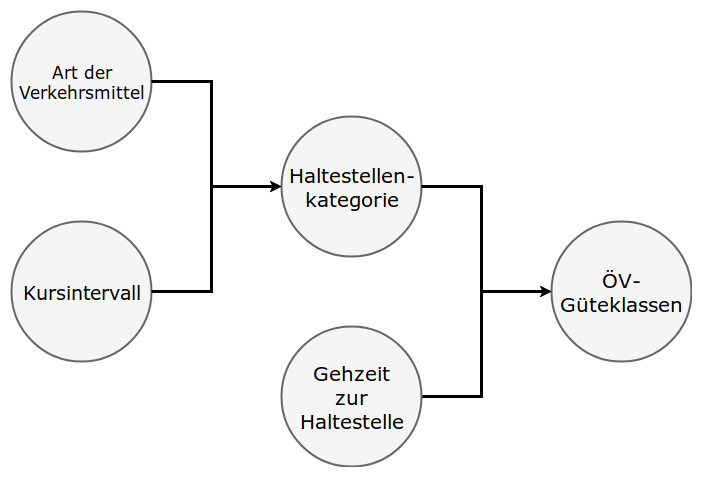
\includegraphics[width=0.7\linewidth]{technicalreport/img/Flow_OeVGK_Brechnung}
    \caption[Schema ÖV-Güteklassen Berechnung]{Schema ÖV-Güteklassen Berechnung}
    \label{fig:Flow_OeVGK_Brechnung}
\end{figure}

\subsubsection{Art der Verkehrsmittel}
\label{Berechnungsmethodik OeVGK18:Art der Verkehrsmittel}
Verkehrsmittel werden in folgende Verkehrsmittelgruppen eingeteilt:

\begin{itemize}[noitemsep]
    \item Verkehrsmittelgruppe A
    \begin{itemize}
        \item Bahnknoten
    \end{itemize}
    \item Verkehrsmittelgruppe B
    \begin{itemize}
        \item Bahnlinie
    \end{itemize}
    \item Verkehrsmittelgruppe C
    \begin{itemize}
        \item Tram, Bus, Postauto, Rufbus, Schiff, Seilbahn
    \end{itemize}
\end{itemize}

\paragraph{Bahnknoten}~\\
Bahnknoten sind Bahnstationen, die entweder einen Anschluss an den nationalen Fernverkehr haben und/oder Bahnlinien in mindestens 6 Richtungen verkehren.

Die Anzahl Richtungen einer Bahnstation wird gezählt als die Anzahl umliegender Bahnstationen, die mit einem beliebigen Zug innerhalb des definierten Zeitbereichs ohne Zwischenhalt erreicht werden können.

\paragraph{Schiffe und Seilbahnen}~\\
Schiffe und Seilbahnen werden nur berücksichtigt, wenn sie ein besiedeltes Wohngebiet erschliessen und nicht ausschliesslich für touristische Zwecke verwendet werden.


\subsubsection{Kursintervall}
\label{Berechnungsmethodik OeVGK18:Kursintervall}
Es sind 3 Stichtage mit jeweils zwei Zeitintervallen zu definieren, welche ausserhalb der Ferienzeit und der touristischen Hochsaison liegen.

\begin{table}[H]
    \centering
    \begin{tabular}[c]{l l}
        \toprule
        \textbf{Stichtag}
                                & \textbf{Zeitintervall}\\
        \midrule
        Werktag
                                & 06:00 -- 20:00 Uhr\\
        Werktag
                                & 20:00 -- 00:00 Uhr\\
        \midrule
        Samstag
                                & 06:00 -- 20:00 Uhr\\
        Samstag
                                & 01:00 -- 04:00 Uhr\\
        \midrule
        Sonntag
                                & 06:00 -- 20:00 Uhr\\
        Sonntag
                                & 01:00 -- 04:00 Uhr\\
        \bottomrule
    \end{tabular}
    \caption{Stichtag und Zeitintervall}
    \label{table:Stichtag und Zeitintervall}
\end{table}

Der Kursintervall $\tau$ einer Haltestelle wird definiert als das "`Doppelte der erwarteten Wartezeit auf die nächste Abfahrt [\ldots] bei zufälligem Zugang im Zeitintervall $I = [a,b)$"'~\cite{visum_manual_formula}.
Es werden nur Abfahrten betrachtet, die innerhalb des definiertem Zeitintervall an der Haltestelle abfahren.

Die Umsetzung dafür geschieht wie folgt:

\begin{tabbing}
Abfahrtszeitpunkte im Zeitintervall $I$: {\hskip 8em} \=    $x_{1 \ldots n}$      \\
Erste Abfahrt nach Zeitpunkt $b$ (nach Fahrplan): \>    $x'$                  \\
Fiktive Abfahrt nach $b$ bei zyklischer Fortsetzung: \> $x'' = x_1 + (b - a)$
\end{tabbing}

Für die Wartezeit am Zeitintervallende wird die Fahrt $x_{n+1} = min\{x', x''\}$ verwendet.

Kursintervall:
\[
    \tau^{a, b} = \frac{1}{b - a} \sum_{i=0}^n \Delta_i
\]

\begin{conditions}
    \Delta_i & $(x_{i+1} - x_i)^2$ {\hskip 2em} für $i \in \{1, \ldots, n - 1\}$ \\
    \Delta_0 & $(x_1 - a)^2$ \\
    \Delta_n & $(x_{n+1} - x_n)^2 - (x_{n+1} - b)^2$
\end{conditions}

\cleardoublepage
\subsubsection{Haltestellenkategorie}
\label{Berechnungsmethodik OeVGK18:Haltestellenkategorie}
Die Haltestellenkategorie I bis VII wird mit folgender Tabelle eruiert:

\begin{table}[H]
    \begin{tabular}[c]{l p{4.0cm} p{4.0cm} p{4.0cm}}
        \toprule
        \textbf{Kursintervall [min]}
                                & \multicolumn{3}{c}{\textbf{Verkehrsmittelgruppe}}\\
        \midrule
        \textbf{}
                                & \textbf{A}
                                & \textbf{B}
                                & \textbf{C}\\
        \textbf{≤ 5}
                                & I
                                & I
                                & II\\
        \textbf{(5, 10]}
                                & I
                                & II
                                & III\\
        \textbf{(10, 20]}
                                & II
                                & III
                                & IV\\
        \textbf{(20, 40]}
                                & III
                                & IV
                                & V\\
        \textbf{(40, 60]}
                                & IV
                                & V
                                & VI\\
        \textbf{> 60}
                                & -
                                & VII
                                & VII\\
        \bottomrule
    \end{tabular}
    \caption{Haltestellenkategorie}
    \label{Haltestellenkategorie}
\end{table}

\subsubsection{Gehzeit zur Haltestelle}
\label{Berechnungsmethodik OeVGK18:Gehzeit zur Haltestelle}
Bei der Berechnung der Gehzeit zu einer Haltestelle ist eine Laufgeschwindigkeit von $1.4 m/s$ anzunehmen und die Strecke entlang des Wege- und Strassennetzes zu berücksichtigen, welche im Folgenden als Horizontaldistanz bezeichnet wird.

Damit man der Topographie gerecht wird, ist als massgebende zu laufende Distanz Leistungsmeter zu verwenden:
\[
    x = 
\begin{cases}
    a + b/0.1 + c/0.15, & \text{wenn } c/d>0.22\\
    a + b/0.1,          & \text{sonst}
\end{cases}
\]
\begin{conditions}
    x   &   Leistungsmeter [m]\\
    a   &   Horizontaldistanz [m]\\
    b   &   positive Steigung in Höhenmeter [m]\\
    c   &   negative Steigung in Höhenmeter [m]\\
    d   &   Horizontaldistanz mit negativer Steigung [m]
\end{conditions}

Die Gehzeit $t$ zur Haltestelle ergibt sich nun aus:
\[ t = \frac{x}{1.4 m/s} \]


\subsubsection{ÖV-Güteklassen}
\label{Berechnungsmethodik OeVGK18:ÖV-Güteklassen}
Die Kombination aus Haltestellenkategorie und Gehzeit zur Haltestelle liefert folgende \acs{ÖV}-Güteklassen-Gruppierung:

\begin{table}[H]
    \begin{tabular}[c]{l p{2.6cm} p{2.6cm} p{2.6cm} p{2.6cm}}
        \toprule
        \textbf{Haltestellenkategorie}
                                & \multicolumn{4}{c}{\textbf{Gehzeit zur Haltestelle [s]}}\\
        \midrule
        \textbf{}
                                & \textbf{≤ 300}
                                & \textbf{(300, 450]}
                                & \textbf{(450, 600]}
                                & \textbf{(600, 900]}\\
        \textbf{I}
                                & Klasse A
                                & Klasse A
                                & Klasse B
                                & Klasse C\\
        \textbf{II}
                                & Klasse A
                                & Klasse B
                                & Klasse C
                                & Klasse D\\
        \textbf{III}
                                & Klasse B
                                & Klasse C
                                & Klasse D
                                & Klasse E\\
        \textbf{IV}
                                & Klasse C
                                & Klasse D
                                & Klasse E
                                & -\\
        \textbf{V}
                                & Klasse D
                                & Klasse E
                                & -
                                & -\\
        \textbf{VI}
                                & Klasse E
                                & -
                                & -
                                & -\\
        \textbf{VII}
                                & Klasse F
                                & -
                                & -
                                & -\\                                
        \bottomrule
    \end{tabular}
    \caption{ÖV-Güteklassen}
    \label{table:ÖV-Güteklassen}
\end{table}

Die Grenze wird bei einem Angebot schlechter als Stundentakt und einem Einzugsgebiet von 300 Sekunden gezogen, da man bei einer weiteren Betrachtung nicht mehr von einer Erschliessung reden kann und so auch nicht ausgewiesen werden soll.




\printglossary[type=main,title=Glossar]

% \ac prints the longform the first time, after that the short
% using \acs always prints the shortform
   
\chapter*{Abkürzungsverzeichnis}\addcontentsline{toc}{chapter}{Abkürzungsverzeichnis}
\begin{acronym}[UVEK] % [] should contain the longest acronym
    \acro{ARE}{Bundesamt für Raumentwicklung}
    \acro{ÖV}{Öffentlicher Verkehr}
    \acro{SN}{Schweizer Norm}
    \acro{ARE}{Bundesamt für Raumentwicklung}
    \acro{UVEK}{Eidgenössisches Departement für Umwelt, Verkehr, Energie und Kommunikation}
\end{acronym}


\cleardoublepage % https://tex.stackexchange.com/a/98995
\phantomsection
\addcontentsline{toc}{chapter}{Literaturverzeichnis}
\bibliographystyle{IEEEtran}
\bibliography{thesis}

\cleardoublepage
\phantomsection
\addcontentsline{toc}{chapter}{Abbildungsverzeichnis}
\listoffigures

\cleardoublepage
\phantomsection
\addcontentsline{toc}{chapter}{Tabellenverzeichnis}
\listoftables

\end{document}
